\section{Use case}
\label{sec:use_case}
Gli \textit{use case} sono uno strumento grafico che permette di analizzare e approfondire i requisiti utente per arrivare a definire i requisiti software del sistema.

\subsection{Descrizione Use Case}

\begin{figure}[H]
    \centering
    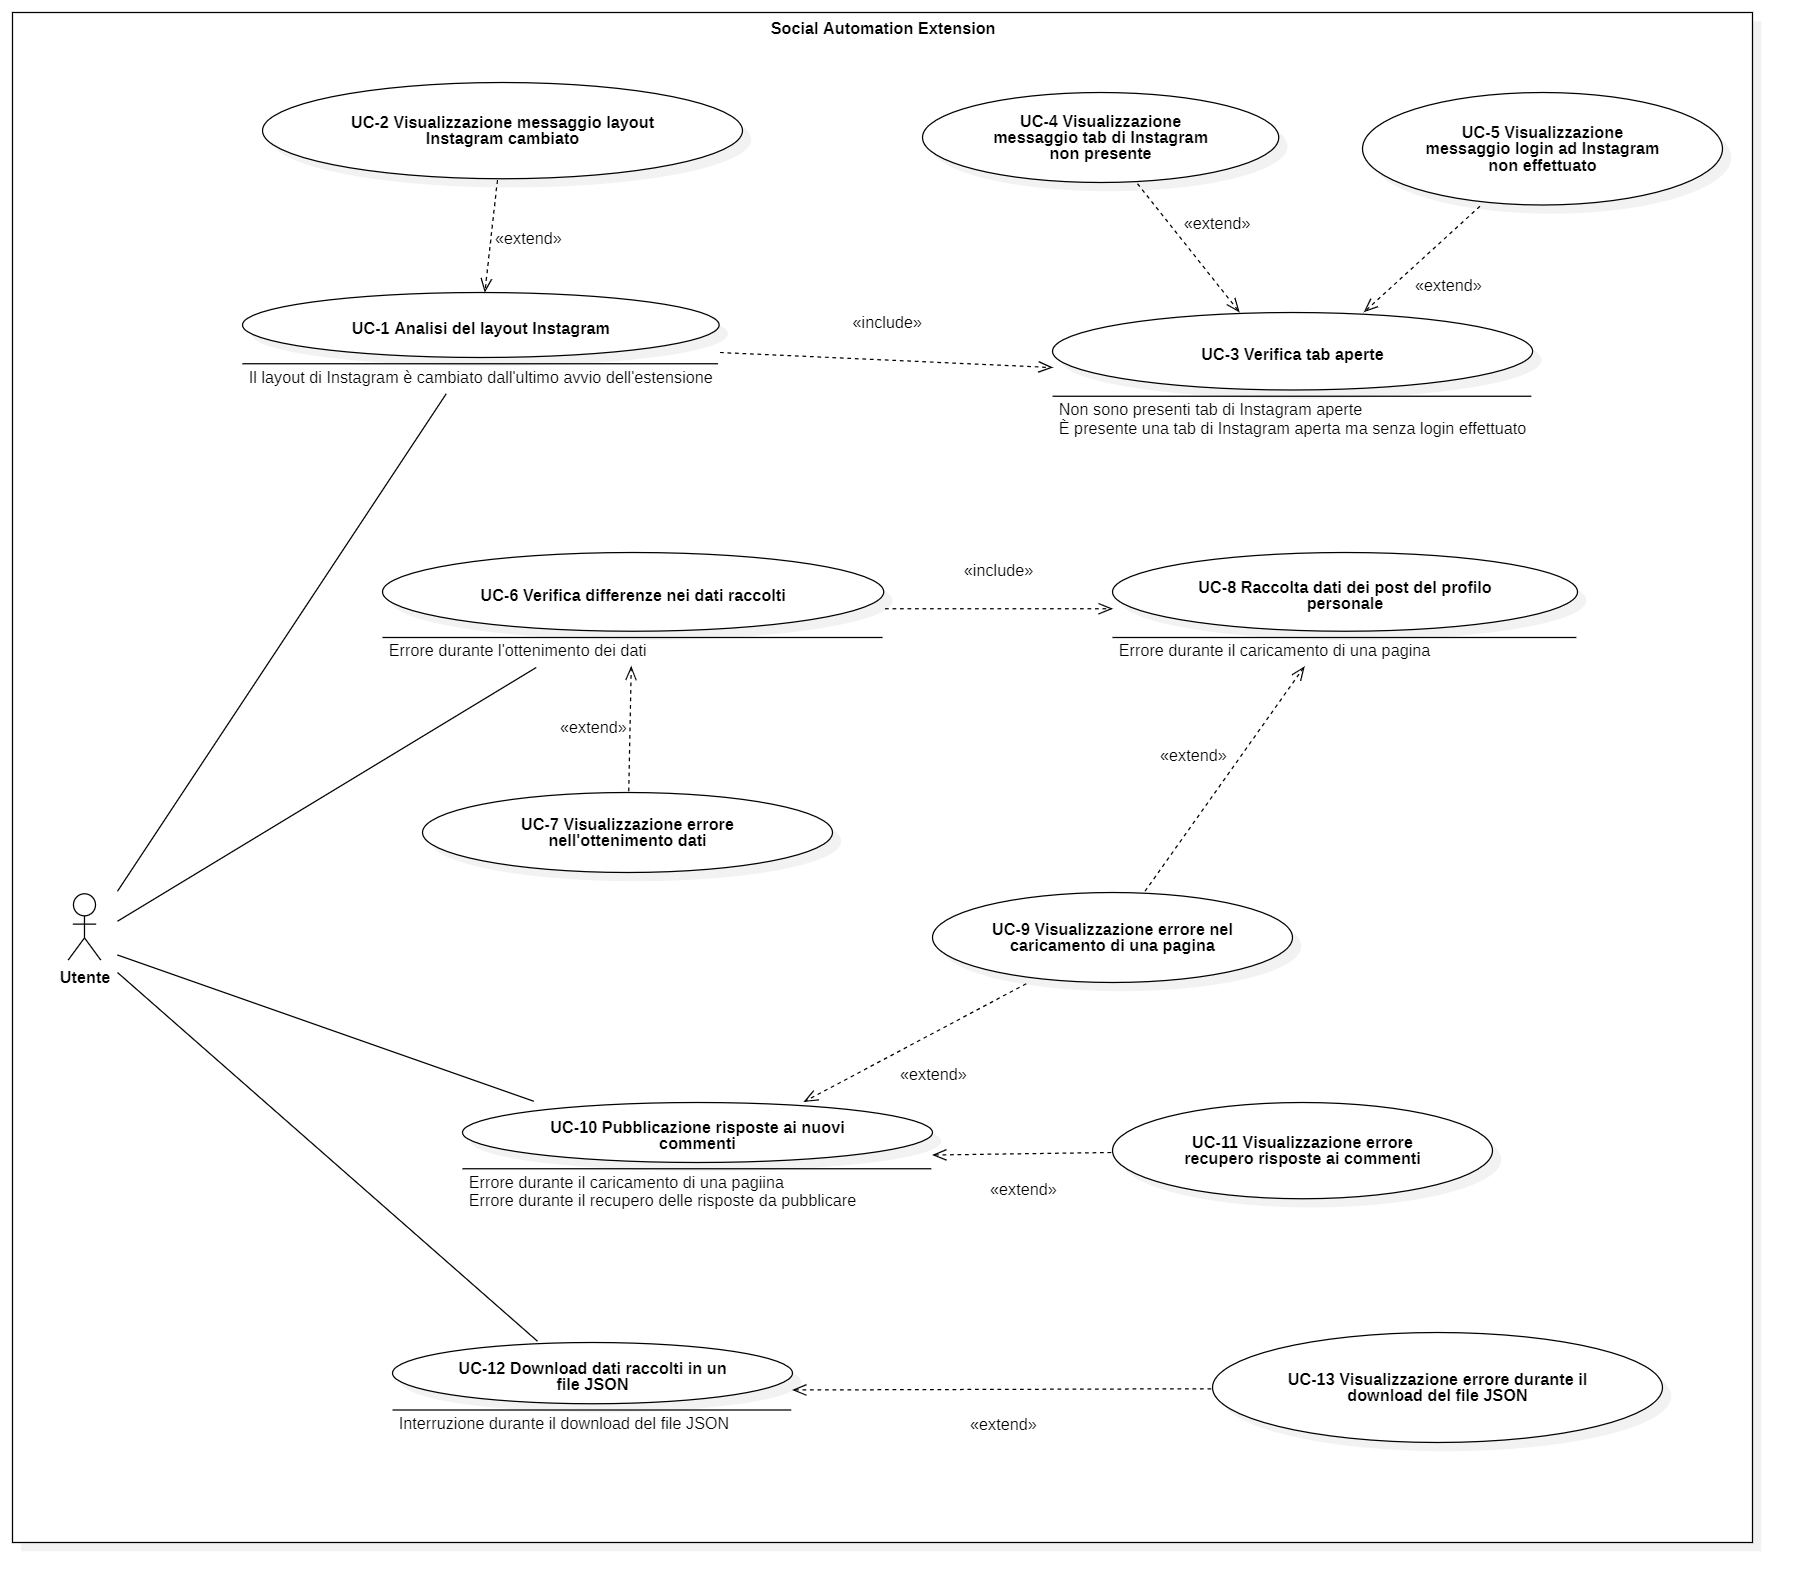
\includegraphics[width=\linewidth]{Sezioni/UseCase/Immagini/Generale.png}
    \caption{Diagramma generale use case}
\end{figure}

\begin{usecase}{UC-1}{Analisi del layout Instagram} 
    \label{uc:UC-1}

    \pre{} 
    
    \post{
        \item Viene visualizzato il pulsante che permette la raccolta dei dati
    }

    \actor{Utente} 

    \trigger{L'utente ha premuto sull'icona dell'estensione Chrome} 

    \inc{\hyperref[uc:UC-3]{UC-3}}

    \base{} 

    \scenario{ 
        \item L'utente preme l'icona per avviare l'estensione Chrome
                    
        \item Il sistema verifica la presenza di una tab Instagram aperta con login effettuato seguendo \hyperref[uc:UC-3]{UC-3}
             
        \item Il sistema esegue l'analisi del layout della pagina di Instagram per rilevare modifiche dovute ad aggiornamenti della piattaforma web

        \item L'utente visualizza il pulsante per effettuare la raccolta dei dati del proprio profilo
    } 

    \subscenario{ 
        \item[3.1] Layout di Instagram variato rispetto l'ultimo utilizzo dell'estensione:
        \begin{itemize}
            \item \hyperref[uc:UC-2]{UC-2}
        \end{itemize}
    } 
  \end{usecase}
  
  \begin{usecase}{UC-2}{Visualizzazione messaggio layout Instagram cambiato} 
    \label{uc:UC-2}

    \pre{
        \item Il sistema ha rilevato modifiche al layout di Instagram dovute a un aggiornamento della piattaforma web
    } 
    
    \post{
        \item Viene visualizzato un messaggio di errore che indica la variazione del layout di Instagram rispetto all'ultimo utilizzo dell'estensione
        \item Non è permessa la raccolta dei dati del proprio profilo
    }

    \actor{Utente} 

    \trigger{Almeno un elemento previsto nel layout di Instagram non è stato trovato} 

    \inc{}

    \base{} 

    \scenario{
        \item Il sistema mostra un messaggio che indica la variazione del layout di Instagram
    } 

    \subscenario{} 
  \end{usecase}

  \begin{usecase}{UC-3}{Verifica tab aperte} 
    \label{uc:UC-3}

    \pre{
        \item Il sistema non ha informazioni riguardo le tab aperte
    } 
    
    \post{
        \item Il sistema ha determinato la presenza di almeno una tab di Instagram aperta e con login effettuato
    }

    \actor{Utente} 

    \trigger{Il sistema deve verificare la presenza di una tab di Instagram con login effettuato per iniziare l'analisi del layout} 

    \inc{}

    \base{} 

    \scenario{
        \item Il sistema verifica la presenza di almeno una tab di Instagram aperta
        \item Il sistema verifica che l'utente abbia già effettuato il login nel proprio profilo
    } 

    \subscenario{
        \item[1.1] Tab di Instagram non presente
        \begin{itemize}
            \item \hyperref[uc:UC-4]{UC-4}
        \end{itemize}
        \item[2.1] Login nel proprio profilo Instagram non effettuato
        \begin{itemize}
            \item \hyperref[uc:UC-5]{UC-5}
        \end{itemize}
    } 
  \end{usecase}

  \begin{usecase}{UC-4}{Visualizzazione messaggio tab di Instagram non presente} 
    \label{uc:UC-4}

    \pre{
        \item Il sistema ha iniziato la verifica delle tab aperte
    } 
    
    \post{
        \item Il sistema ha determinato l'assenza di una tab di Instagram aperta
        \item L'utente è a conoscenza dei requisiti per utilizzare le funzionalità dell'estensione
    }

    \actor{Utente} 

    \trigger{Il sistema non ha trovato tab di Instagram aperte} 

    \inc{}

    \base{} 

    \scenario{
        \item Il sistema mostra un messaggio che indica la necessità di aprire una tab di Instagram ed effettuare il login
    } 

    \subscenario{} 
  \end{usecase}

  \begin{usecase}{UC-5}{Visualizzazione messaggio login a Instagram non effettuato} 
    \label{uc:UC-5}

    \pre{
        \item Il sistema ha determinato la presenza di almeno una tab di Instagram aperta
    } 
    
    \post{
        \item Il sistema ha determinato che l'utente non ha effettuato il login al suo profilo Instagram
        \item L'utente è a conoscenza della necessità di effettuare il login per poter utilizzare le funzionalità dell'estensione
    }

    \actor{Utente} 

    \trigger{Il sistema ha rilevato una scheda di Instagram aperta, ma senza che sia effettuato l'accesso a un profilo} 

    \inc{}

    \base{} 

    \scenario{
        \item Il sistema mostra un messaggio che indica la necessità di effettuare il login al proprio profilo Instagram
    } 

    \subscenario{} 
  \end{usecase}

  \begin{usecase}{UC-6}{Verifica differenze nei dati raccolti} 
    \label{uc:UC-6}

    \pre{
        \item Il sistema ha traccia dei dati raccolti nell'ultima esecuzione
        \item Il sistema termina la nuova raccolta dati con successo
    } 
    
    \post{
        \item Il sistema verifica se, nell'ultima raccolta, sono stati acquisiti nuovi dati e informa l'utente
    }

    \actor{Utente} 

    \trigger{L'utente ha avviato l'analisi dei dati del proprio profilo} 

    \inc{\hyperref[uc:UC-8]{UC-8}}

    \base{} 

    \scenario{
        \item L'utente richiede di analizzare i dati del proprio profilo
        \item Il sistema tiene traccia degli ultimi dati raccolti
        \item Il sistema effettua la raccolta dei nuovi dati seguendo \hyperref[uc:UC-8]{UC-8}
        \item Il sistema calcola le differenze tra i nuovi dati raccolti e i dati precedenti
        \item L'utente visualizza un messaggio che indica se sono presenti nuovi dati 
    } 

    \subscenario{
        \item[2.1] Errore interno durante l'ottenimento dei dati acquisiti nell'ultima raccolta
        \begin{itemize}
            \item \hyperref[uc:UC-7]{UC-7}
        \end{itemize}
        \item[4.1] Errore interno durante l'ottenimento dei dati acquisiti nella raccolta appena terminata
        \begin{itemize}
            \item \hyperref[uc:UC-7]{UC-7}
        \end{itemize}
    } 
  \end{usecase}

  \begin{usecase}{UC-7}{Visualizzazione errore nell'ottenimento dei dati} 
    \label{uc:UC-7}

    \pre{
        \item Avviene un errore interno al sistema durante l'ottenimento dei dati gestiti da esso
    } 
    
    \post{
        \item L'utente è a conoscenza dell'errore interno avvenuto
    }

    \actor{Utente} 

    \trigger{Il sistema riscontra un errore interno durante l'ottenimento dei dati} 

    \inc{}

    \base{} 

    \scenario{
        \item Il sistema notifica all'utente, mediante un messaggio di errore, la causa dell'anomalia
    } 

    \subscenario{} 
  \end{usecase}

  \begin{usecase}{UC-8}{Raccolta dati dei post del profilo personale} 
    \label{uc:UC-8}

    \pre{
        \item L'analisi del layout di Instagram è terminata con successo
    } 
    
    \post{
        \item Il sistema ha salvato i nuovi dati relativi ai post del profilo Instagram personale
    }

    \actor{Utente} 

    \trigger{L'utente ha premuto il pulsante per iniziare la raccolta dati} 

    \inc{}

    \base{} 

    \scenario{
        \item L'utente preme il pulsante per avviare una nuova raccolta dati
        \item Il sistema naviga il profilo dell'utente e raccoglie per ogni post: URL, numero, caption, src immagine, numero di like e lista dei commenti (autore e testo)
        \item Il sistema salva i dati raccolti
    } 

    \subscenario{
        \item[2.1] Tempo di caricamento eccessivo della pagina di un post
        \begin{itemize}
            \item \hyperref[uc:UC-9]{UC-9}
        \end{itemize}
    } 
  \end{usecase}

  \begin{usecase}{UC-9}{Visualizzazione errore nel caricamento di una pagina} 
  \label{uc:UC-9}

    \pre{
        \item Il caricamento di una pagina di un post durante la raccolta dati richiede un tempo eccessivo
    } 
    
    \post{
        \item L'utente è a conoscenza del problema riscontrato
    }

    \actor{Utente} 

    \trigger{Il tempo di caricamento della pagina di un post supera il timeout impostato} 

    \inc{}

    \base{} 

    \scenario{
        \item Viene mostrato un messaggio di errore che informa l'utente su quanto accaduto
    } 

    \subscenario{} 
  \end{usecase}

  \begin{usecase}{UC-10}{Pubblicazione risposte ai nuovi commenti} 
  \label{uc:UC-10}

    \pre{
        \item Il sistema ha terminato una raccolta dati e confrontando i risultati con la raccolta precedente ha rilevato differenze
    } 
    
    \post{
        \item Vengono pubblicate le risposte automatiche ai nuovi commenti rilevati
    }

    \actor{Utente} 

    \trigger{L'utente ha richiesto di pubblicare le risposte ai nuovi commenti rilevati} 

    \inc{}

    \base{} 

    \scenario{
        \item L'utente preme il pulsante per pubblicare le risposte automatiche
        \item Il sistema recupera una risposta da associare per ogni nuovo commento rilevato
        \item Il sistema ricerca ogni commento all'interno dei post e pubblica la risposta
        \item L'utente visualizza un messaggio di conferma della pubblicazione delle risposte
    } 

    \subscenario{
        \item[3.1] Errore durante il recupero delle risposte da pubblicare ai commenti
        \begin{itemize}
            \item \hyperref[uc:UC-11]{UC-11}
        \end{itemize}
        \item[3.1] Tempo di caricamento eccessivo della pagina di un post
        \begin{itemize}
            \item \hyperref[uc:UC-9]{UC-9}
        \end{itemize}
    } 
  \end{usecase}

  \begin{usecase}{UC-11}{Visualizzazione errore recupero risposte ai commenti} 
  \label{uc:UC-11}

    \pre{
        \item Avviene un errore interno al sistema durante il recupero delle risposte da pubblicare ai commenti
    } 
    
    \post{
        \item L'utente è a conoscenza dell'errore interno avvenuto
    }

    \actor{Utente} 

    \trigger{Il sistema riscontra un errore interno durante l'ottenimento delle risposte da pubblicare} 

    \inc{}

    \base{} 

    \scenario{
        \item Il sistema notifica all'utente, mediante un messaggio di errore, la causa dell'anomalia
    } 

    \subscenario{} 
  \end{usecase}

  \begin{usecase}{UC-12}{Download dati raccolti in un file JSON} 
  \label{uc:UC-12}

    \pre{
        \item Il sistema ha terminato una raccolta dati e confrontando i risultati con la raccolta precedente ha rilevato differenze
    } 
    
    \post{
        \item Viene scaricato un file JSON contenente i nuovi dati raccolti
    }

    \actor{Utente} 

    \trigger{L'utente ha richiesto il download del file JSON con i nuovi dati raccolti} 

    \inc{}

    \base{} 

    \scenario{
        \item L'utente preme il pulsante per scaricare il file JSON
        \item Il sistema avvia il download
        \item L'utente visualizza un messaggio di successo del download del file
    } 

    \subscenario{
        \item[2.1] Interruzione durante il download del file JSON richiesto
        \begin{itemize}
            \item \hyperref[uc:UC-13]{UC-13}
        \end{itemize}
    } 
  \end{usecase}

  \begin{usecase}{UC-13}{Visualizzazione errore durante il download del file JSON} 
  \label{uc:UC-13}

    \pre{
        \item Avviene un'interruzione durante il download del file JSON
    }

    \post{
        \item L'utente è a conoscenze dell'interruzione avvenuta
    }

    \actor{Utente} 

    \trigger{Il sistema rileva un'interruzione durante il download del file} 

    \inc{}

    \base{} 

    \scenario{
        \item Il sistema comunica all'utente, mediante un messaggio di errore, che si è verificata un'interruzione
    } 

    \subscenario{} 
  \end{usecase}

  

